% User guide: http://mirrors.ctan.org/macros/latex/contrib/bookcover/bookcover.pdf

\documentclass[
    coverwidth=21cm,  % largura da página
    coverheight=29.7cm, % altura da página
    spinewidth=12mm,  % grossura
%    flapwidth=8cm,    % orelha 
%    wrapwidth=5mm,    % linha vermelha - orelha 
%    trimmed % Show only trimmed part!
    ]{bookcover}

%\bookcovertrimmedpart{front} % Trimmed part is the front cover
%\bookcovertrimmedpart{back} % Trimmed part is the back cover
%\bookcovertrimmedpart{spine} % Trimmed part is the spine

%\usepackage[portuguese]{babel}

\usepackage{graphicx}
\usepackage{adjustbox}

\newbookcovercomponenttype{center rotate}{
    \vfill
    \centering
    \rotatebox[origin=c]{-90}{#1}
    \vfill}

\usepackage[outline]{contour}% It doesn't work with xelatex and lualatex
\contourlength{1pt}
\usepackage[english]{babel}
\usepackage{kantlipsum,microtype}

\usepackage{url}
\usepackage[colorlinks=true,linkcolor=blue,urlcolor=black,citecolor=black,pdfborder={0 0 0}]{hyperref}

\begin{document}

\begin{bookcover}

% Remark
%\begin{bookcoverelement}{center}{above front}
%    \textcolor{blue}{A dust jacket example}
%\end{bookcoverelement}

% Background color on the whole cover
\begin{bookcoverelement}{color}{bg whole}
    green!10
\end{bookcoverelement}

% Background picture on the whole cover without flaps
\begin{bookcoverelement}{picture}{bg whole without flaps}
./figures/img2.png
\end{bookcoverelement}
% \begin{bookcoverelement}{picture}{bg whole without flaps, scale=1.5}
%   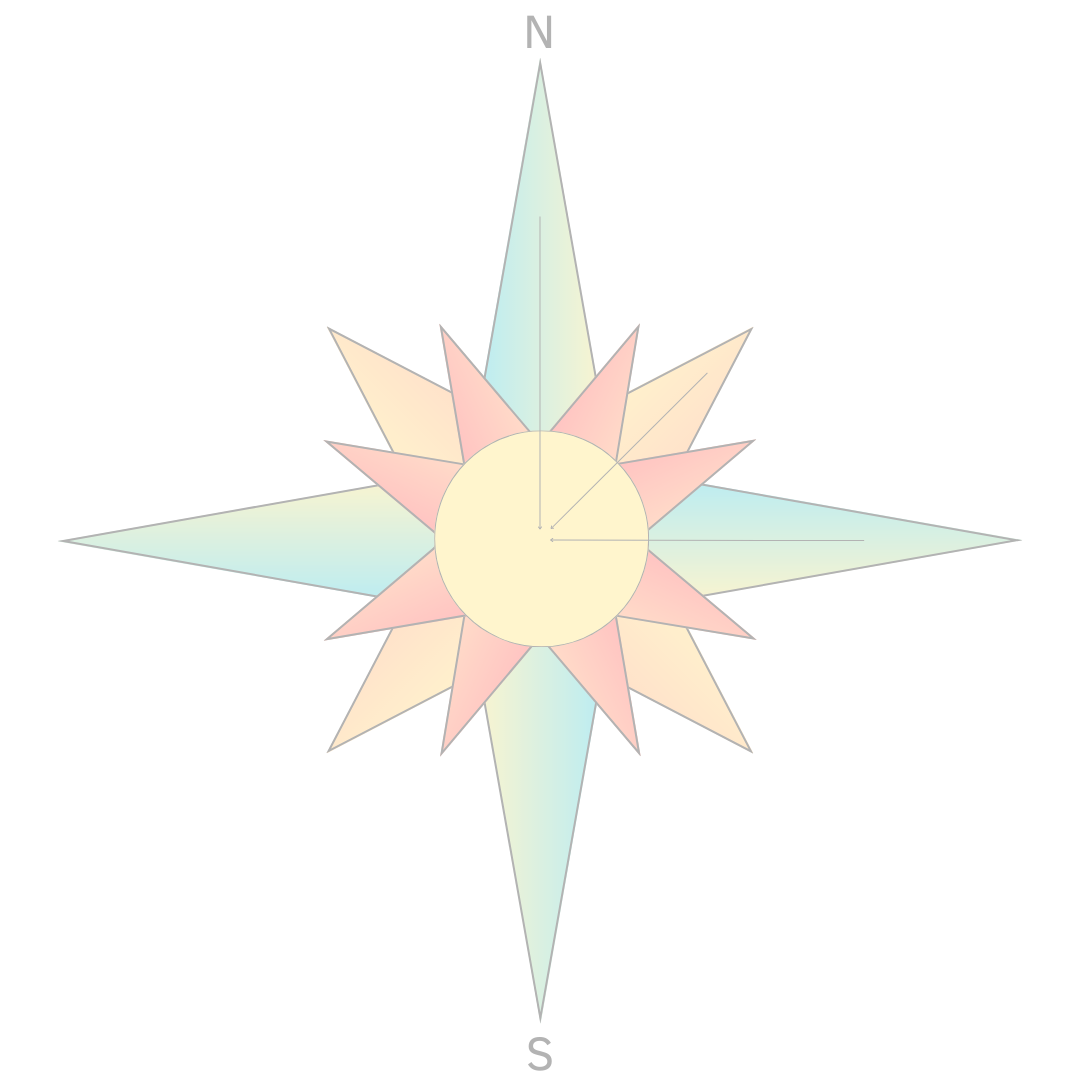
\includegraphics[width=\textwidth]{figures/img3.png}
% \end{bookcoverelement}

% Transparent areas on the back cover
\begin{bookcoverelement}{tikz}{bg back and wrap}
    \fill[opacity=0.3,white] 
    (0,0) rectangle (25mm,\partheight) 
    (part.north east) rectangle ([xshift=-2cm]part.south east);
\end{bookcoverelement}

% Transparent areas on the front cover
\begin{bookcoverelement}{tikz}{bg front and wrap}
    \fill[opacity=0.3,white] 
    (0,0) rectangle (20mm,\partheight) 
    (part.north east) rectangle ([xshift=-25mm]part.south east);
\end{bookcoverelement}

% Picture on the front cover behind the title
\begin{bookcoverelement}{center}{front}
    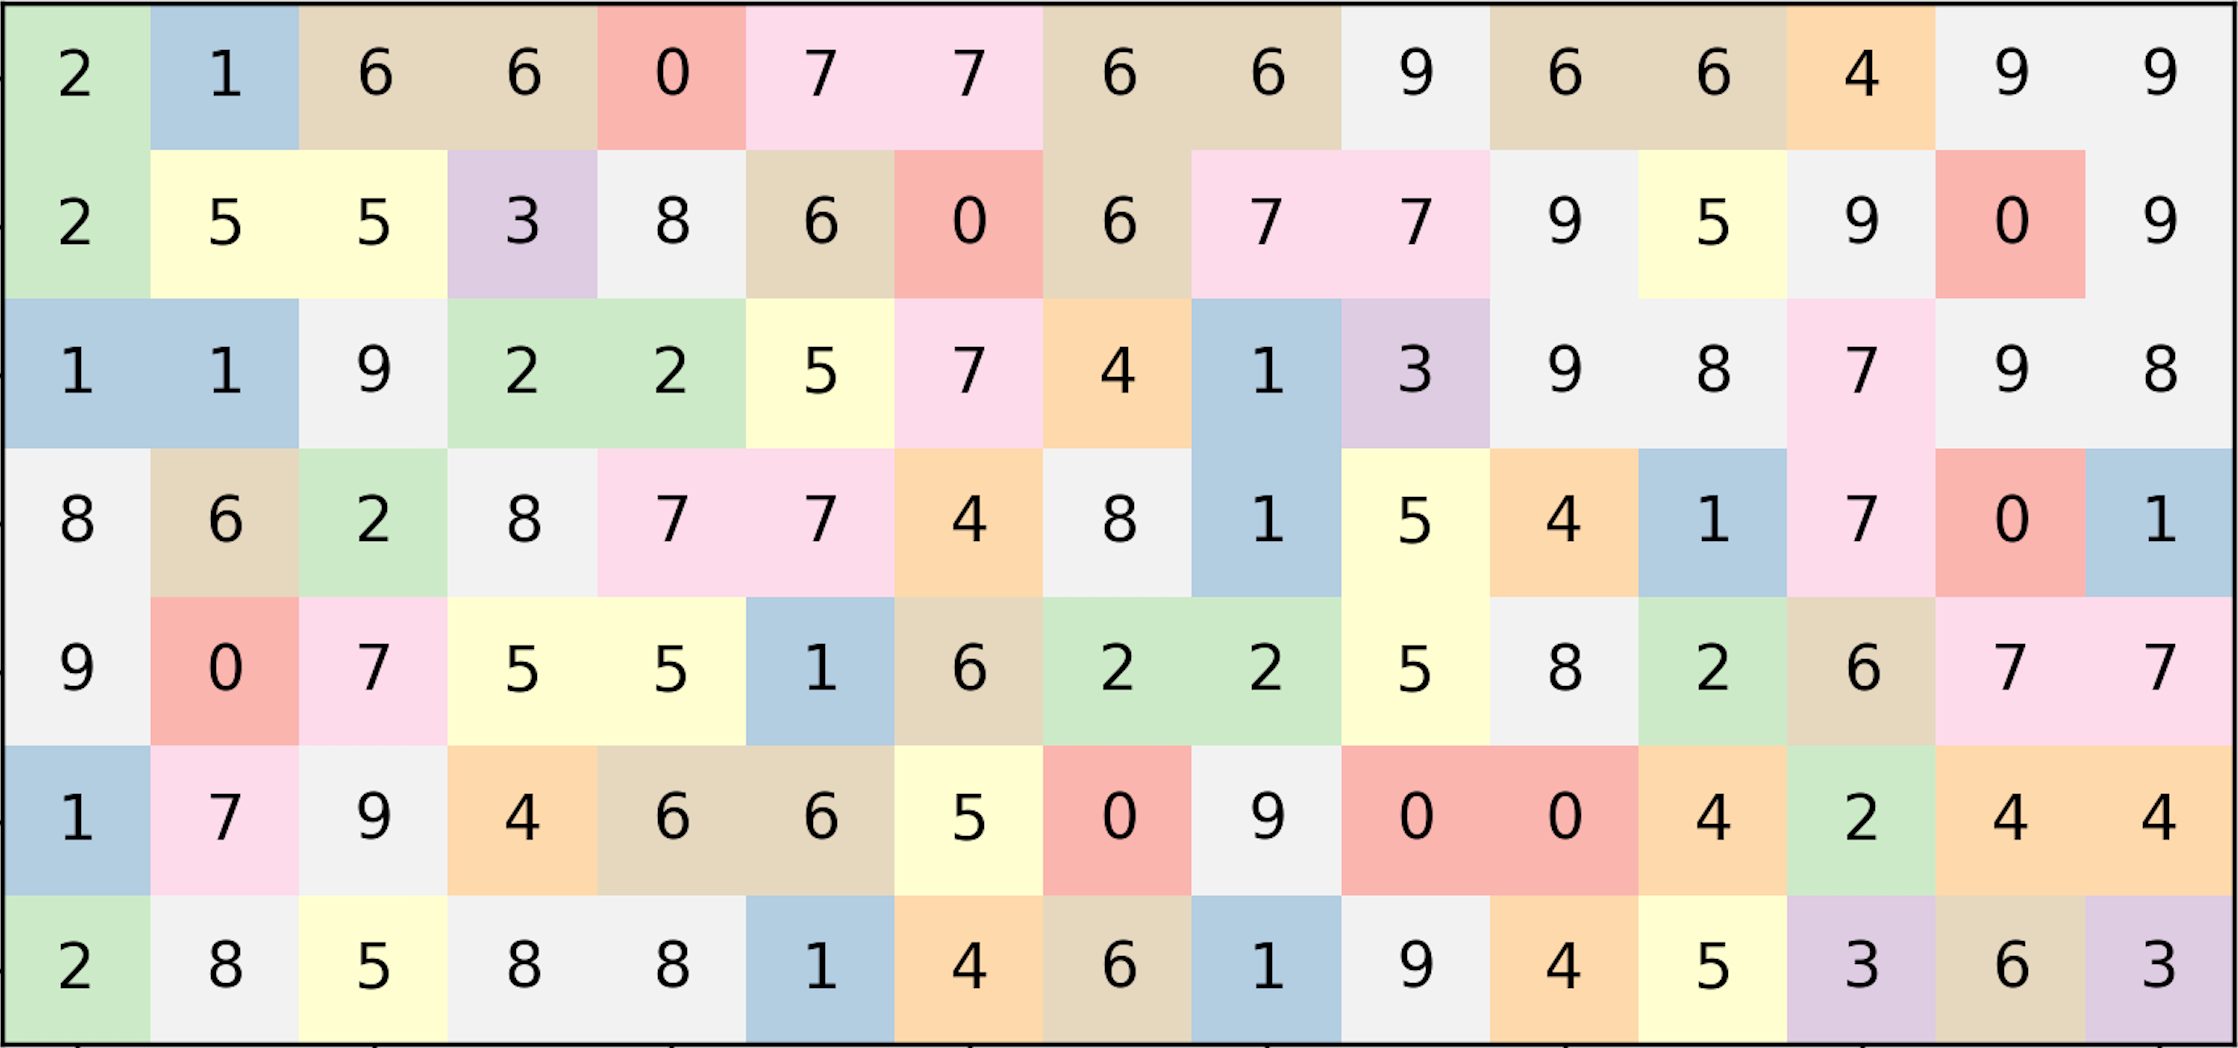
\includegraphics[width=.2\textwidth]{./figures/frente.png}
\end{bookcoverelement}

% Author and title on the front cover
\begin{bookcoverelement}{normal}{front}[,,,3cm]
    \centering
    \color{yellow}\sffamily\bfseries
    \resizebox{!}{5mm}{\contour{green!30!black!80}{Francisco de Assis Zampirolli}}\\[42mm]    
\resizebox{!}{7mm}{\contour{green!30!black!80}{MCTest}}\\[128mm]
    \resizebox{!}{6mm}{\contour{green!30!black!80}{Como Criar e Corrigir Exames}}\\[8mm]
    \resizebox{!}{6mm}{\contour{green!30!black!80}{Parametrizados Automaticamente}}\\[33mm]
   
{\centering
%
\includegraphics[width=.06\textwidth]{./figures/ufabc.png}\\
\color{green!30!black!80}\Large 2a Edição \\ 2024}

\end{bookcoverelement}


% Title on the spine
\begin{bookcoverelement}{center rotate}{spine}
    \color{yellow}\sffamily\bfseries
    \resizebox{!}{3.1mm}{\contour{green!30!black!80}{MCTest: Como Criar e Corrigir Exames Parametrizados Automaticamente\hspace{6,7cm}}}
\end{bookcoverelement}

\begin{bookcoverelement}{center rotate}{spine}
    \color{yellow}\sffamily\bfseries
    \resizebox{!}{3.7mm}{\contour{green!30!black!80}{\hspace{10,5cm}Francisco de Assis Zampirolli}}
\end{bookcoverelement}

% Text on the back cover
\begin{bookcoverelement}{normal}{back}[2cm,2cm,2cm,2cm]
    \color{white}%\kant[1]
\end{bookcoverelement}

% Text and picture on the front flap
\begin{bookcoverelement}{normal}{front flap}[10mm,10mm,10mm,10mm]
    \color{black}\large
A avaliação de muitos estudantes é um desafio para os professores em todos os níveis de ensino. Para ame\-nizar essa tarefa, este livro apresenta o MCTest, um sistema de código aberto para elaboração e correção de exa\-mes. Esse sistema oferece questões parametrizadas e exa\-mes indivi\-dualizados que podem ser utilizados por várias turmas simulta\-neamente, cada uma com exames diferentes, mas com os mesmos níveis de dificuldade.
%
Embora a ideia inicial fosse utilizar o sistema para corrigir exames em processos seletivos de mi\-lhares de candidatos para a Especia\-lização em Tecnologias e Sistemas de Informação da UFABC desde 2012, com questões de múltipla escolha, o sistema evoluiu considera\-velmente para uma versão web completa. Veja um exemplo em \url{mctest.ufabc.edu.br}.
%
O foco deste livro é ensinar como criar exames parametrizados para correção automática, inclusive com Exercícios de Programação (EP) para correção no Moodle, utilizando o \textit{plugin} VPL (\textit{Virtual Programming Lab}). Esses EPs são criados por meio da fusão de tex\-tos \LaTeX{} e códigos Python.
%
No entanto, antes de elaborar esses EPs, é necessário discutir como navegar no sistema usando um dos três tipos de usuários: administrador, coordenador de disciplina e professor. Um professor sem habilidades de programação também pode usar o MCTest para criar exames com questões estáticas, onde a única variação é a seleção aleatória de perguntas e alternativas. %\kant[2]
    %\vfill
    %{\centering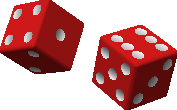
\includegraphics{./figures/bookcover-dice.pdf}\par}
\end{bookcoverelement}

% Text on the back flap
\begin{bookcoverelement}{normal}{back flap}[10mm,10mm,10mm,10mm]
    \color{black}\large
    Francisco de Assis Zampirolli é professor na Universidade Federal do ABC (UFABC) desde 2008, com graduação em Matemática pela UFES, mestrado em Matemática Aplicada pelo IME/USP, e Doutorado em Engenharia de Computação pela UNICAMP. Com mais de 25 anos de experiência em ensino de computação, foi o criador do MCTest, um software livre amplamente utilizado por professores e mi\-lhares de estudantes para geração e correção automática de exames. Suas principais áreas de pesquisa concentram-se em Processamento Digital de Imagens, Geração Automática de Documentos e Ensino de Computação.
Além do trabalho no ensino de computação, também participa ativamente de projetos de pesquisa e extensão. Essas atividades na UFABC incluem o uso do MCTest:
(1) na Especialização em Tecnologias e Sistemas de Informação;
(2) no oferecimento de um pré-vestibular gratuito para a comunidade carente da região do ABC;
(3) em disciplinas na graduação e pós-graduação.
%\kant[3]
     \vfill
    \hspace{5mm}{\centering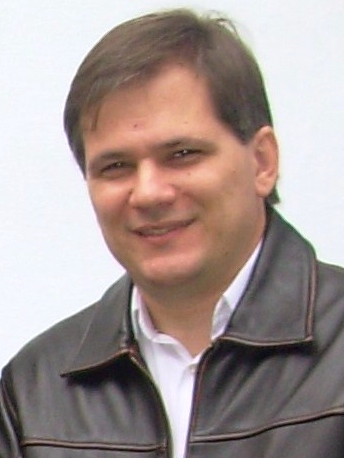
\includegraphics[width=.08\textwidth]{./figures/zampirolli.png}}
\end{bookcoverelement}


\begin{bookcoverelement}{normal}{back}[20mm,20mm,20mm,20mm]
\color{black}\Large
Este livro ensina como elaborar e avaliar exames contendo questões, com destaque especial para as questões paramétricas, um tipo específico de questão que incorpora valores aleatórios em sua formulação. Além disso, o livro compartilha as melhores experiências adquiridas ao longo dos últimos 12 anos em avaliações automatizadas, que trouxeram vantagens tanto para os professores quanto para milhares de estudantes da UFABC. \\[3mm]

\textbf{Exemplo:} Na área de Lógica de Programação, o livro apresenta várias questões paramétricas, como um programa que retorna a matriz ``nordeste maior'' a partir da matriz de entrada, conforme ilustrado neste exemplo na capa. Por outro lado, em Processamento Digital de Imagens, a solução é alcançada por meio da adaptação de erosão ou dilatação com um elemento estruturante de tamanho $3\times 3$. \\[95mm]

\textbf{Obs.:} Esta questão possui $16$ variações, sendo $8$ relacionadas às direções cardeais e as opções de maior ou menor. Além disso, é possível variar as dimensões da matriz e seus respectivos valores. Para disciplinas mais avançadas, é possível aumentar a vizinhança, por exemplo, para $5\times 5$ ou $7\times 7$, criando ainda mais variações.\\[8mm]

    {\centering 
    
\includegraphics[height=27mm,width=25mm]{./figures/qrcode.png}\hfill
    
\includegraphics[height=20mm,width=35mm]{./figures/barcode-impresso.png}
    }
\end{bookcoverelement}
% incluir fundo transparente
% https://www.peko-step.com/pt/tool/alphachannel.html
% https://www.barcode-generator.de/pt/criar-isbn

% Picture on the front cover behind the title
\begin{bookcoverelement}{center}{back}
    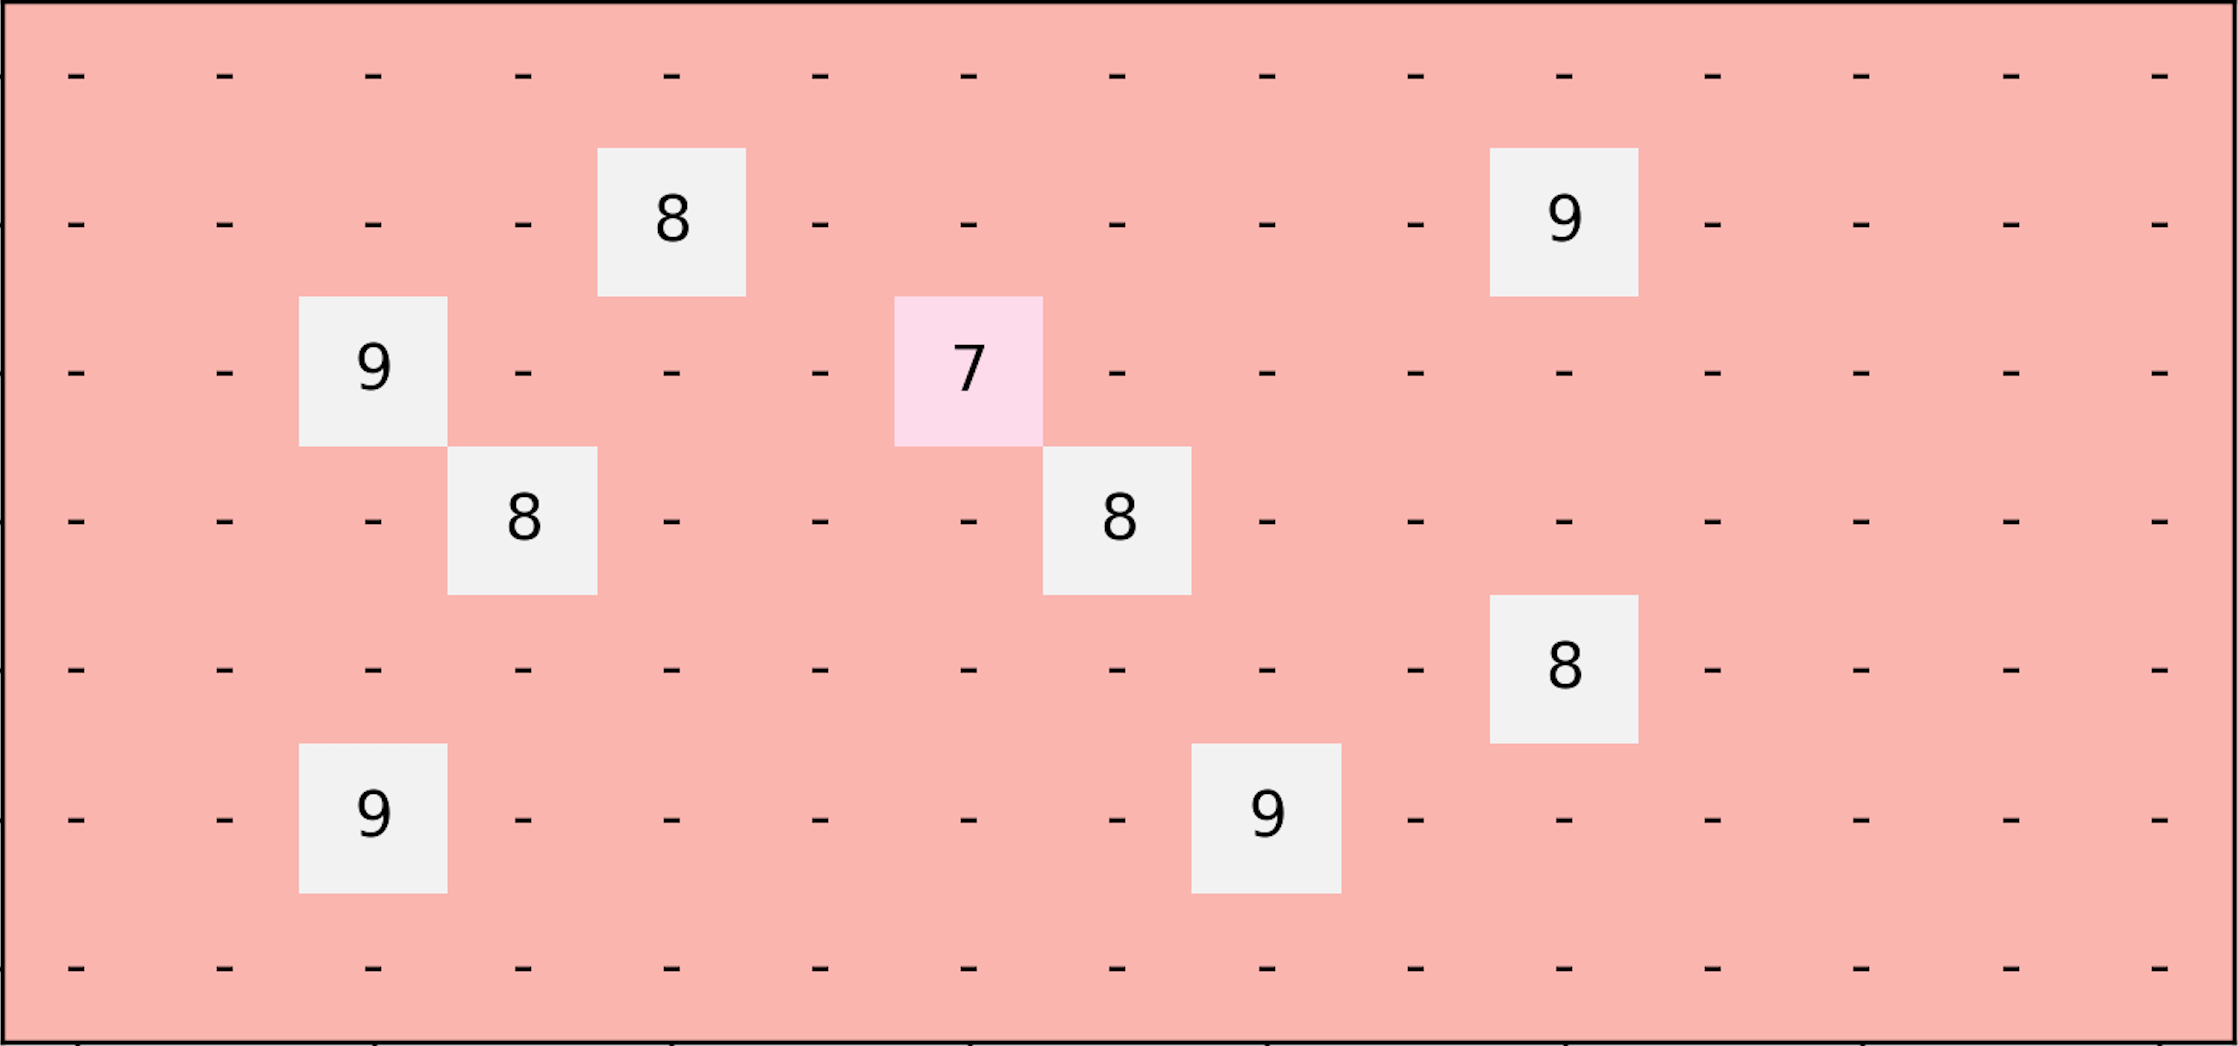
\includegraphics[width=.2\textwidth]{./figures/verso.png}
\end{bookcoverelement}

\end{bookcover}

\end{document}
